\documentclass[14pt]{article}
\usepackage{fullpage,enumitem,amsmath,amssymb,titlesec, xcolor, amsthm, listings, lstautogobble, graphicx}
\usepackage{tikz}
\titleformat*{\section}{\Large\bfseries\color{blue}\filcenter}
\titlespacing*{\subsection}{-1em}{*2}{*0}
\titleformat*{\subsection}{\bfseries\large\color{blue}}
\usepackage{indentfirst}
\setlength\parindent{24pt}
\newtheorem{theorem}{Theorem}
\lstset{
	keywordstyle=\color{blue},
	basicstyle=\scriptsize\ttfamily,
	commentstyle=\ttfamily\itshape\color{gray},
	stringstyle=\ttfamily,
	showstringspaces=false,
	breaklines=true,
	frameround=ffff,
	frame=single,
	rulecolor=\color{black},
	autogobble=true
}



\begin{document}
	
	\title{\color{blue}\Huge \textbf{Assignment-2}} 
	\date{\Large Design and Analysis of Algorithms}
	\author{Rachit Parikh (CRS-2101) -- \texttt{rachitparikh2016@gmail.com}}
	
	\maketitle
	\textbf{Disclaimer :} I declare that all the work presented in this assignment is my own work and I have only consulted the internet when it was absolutely necessary. I have tried adding C++/Python code to almost every solution so if you want to check the codes, you can create a main method and check it for any test case. I have not added correctness proofs for known algorithms like binary search, count sort, radix sort, etc. I have also taken certain assumptions (Eg : I have taken time complexity for radix sort directly in the 2nd question).
	
	\noindent
	\rule{\linewidth}{0.4pt}
	
	\section*{\underline{Q-6}}
		\noindent
		To prove the necessary condition we will need to prove another property which will serve as a stepping stone for the proof.
		\begin{theorem}
			\label{theorem-1}
			For an array $A$ of $n$ numbers (with $curr\_max$ and $curr\_min$ known), add any 2 arbitrary numbers to it and name this new array $A'$. To update the new $min(A')$ and $max(A')$ elements, it would take at least 3 comparisons.
		\end{theorem}
		\begin{proof}
			Let $a$ and $b$ be the new elements to be added to $A$. We will try to prove this theorem by contradiction. Assume that we can update the new $min$ and $max$ elements with 2 comparisons. Now, we have to decide which 2 comparisons should be made to determine the $ new\_min $ and $ new\_max $. We have the following available variables to make comparisons : $ curr\_max, curr\_min, a, b $ and elements of array $A$. But comparing with elements of $A$ apart from $curr\_min$ and $curr\_max$ would not help us in any way to determine the $new_min$ and $new_max$. So, we will stick with $curr\_min, curr\_max, a$ and $b$. \\
			Since we already know the ordering of $curr\_max$ and $curr\_min$ (i.e $curr\_min \leq curr\_max$) we would pick up other pair of combinations to compare. Now we will take cases (two comparisons). Let us denote comparison between $a$ and $b$ as $ [a:b] $.
			\begin{itemize}
				\item Compare $a$ with $b$, let their minimum be $c$ and their maximum be $d$. Now compare $c$ with $curr\_min$. Here two things can happen, either $c < curr\_min$ or $c \geq curr\_min$. If the first case occurs, then we have discovered the $new\_min$, if the latter occurs, then we have $new\_min = curr\_min$. But there is no clear information about the $new\_max$, since both $d$ and $curr\_max$ can be the $new\_max$. For this we will need another comparison of $d$ with $curr\_max$, but we have already exhausted 2 comparisons : $(1) [a:b]$ and $(2) [c:curr\_min]$. (The same thing happens if we take $max(a, b)$ instead of $c$ and compare it with $curr\_max$ first). So, in this sequence of comparison operations we need more than 2 comparisons to determine the $new\_min$ and $new\_max$.
				
				\item Compare $a$ with $curr\_min$, let their minimum be $s$, can we infer that $new\_min = s$?. No, we cannot do it that easily. If it were possible then the world would break and we would be controlled by SkyNet!! It cannot happen because we have not checked with $b$. If it happens that $b < a$, then there is a possibility that $new\_min = b$. So, it would become necessary to take $min(curr\_min, a, b)$ to find the $new\_min$. But if we do that we will exhaust our 2 comparison criteria and we would not be able to find $new\_max$ if that happens because another comparison would be required with $curr\_max$. (The similar argument suffices for the case where we would compare with $curr\_max$ first). 
			\end{itemize}
			We have considered all the non-trivial cases here and we can find that it is not possible to determine the $new\_min$ and $new\_max$ within 2 comparisons. But is it possible to do it in 3 comparisons? It is possible, consider the first case where we compared $a$ and $b$ first. Let their minimum be $c$ and maximum be $d$. After this, do $[curr\_max : d]$ and $[curr\_min : c]$. Here with 3 comparisons we are able to determine the $new\_min$ and $new\_max$. Hence ,we can conclude that at least 3 comparisons are required when we add 2 new elements to the array.
		\end{proof}
		Using the statement of \ref{theorem-1}, we can prove the necessary condition for number of comparisons required to find the $max$ and $min$ elements of an array.
		
		\begin{theorem}
			Number of comparisons "necessary" to find both the minimum and maximum elements of an array of n elements is $\left \lceil \dfrac{3n}{2} \right\rceil - 2$
		\end{theorem} 
		\begin{proof}
			We will use strong induction to prove this statement. We will first prove this statement for the base case $n=2$ and also assume in the induction step that the case holds for all $n \leq k$ and prove the statement for $k+1$.\\
			\linebreak
			For $n=2$, we have only two elements $x$ and $y$. We will need minimum one comparison to find out the maximum and minimum elements because without making any comparisons we cannot guess which element is bigger/smaller than the other with probability 1. 
			$$\left \lceil \dfrac{3n}{2} \right\rceil - 2 = \left \lceil 3\right \rceil - 2 = 1$$
			\linebreak
			Induction step : Assume that the statement holds for $n \leq k$.\\
			\linebreak
			Now, for $k+1$, we will use \ref{theorem-1}. The minimum number of comparisons required when two elements are added into an array of $k-1$ elements is 3. Let $T(k)$ denote the minimum number of comparisons required to find minimum and maximum in an array of $k$ elements. Then by \ref{theorem-1}, we have 
			\begin{align*}
				T(k+1) \geq T(k-1) + 3\\
				T(k+1) \geq \left \lceil \dfrac{3(k-1)}{2} \right\rceil - 2 + 3\\
				\implies T(k+1) \geq \left \lceil \dfrac{3(k-1)}{2} + 3\right\rceil - 2\\
				\therefore T(k+1) \geq \left \lceil \dfrac{3(k+1)}{2}\right\rceil - 2\\
			\end{align*}
		Hence proved!
		\end{proof}
		We have proved the necessary condition for the number of comparisons, now we proceed to sufficiency condition.\\
		\linebreak
		For sufficiency, we just need to show an algorithm that can find minimum and maximum element of an array within the given number of comparisons. The python code of the algorithm is as follows:
		\newpage
		\begin{lstlisting}[language=Python]
			
			def get_max_min(A):
				n = A.size()
				start = 0
				
				# If array size is odd, initiate both max and min as first element
				# Else we make a comparison and initialize appropriately
				
				if n & 1 == 0:
					max_so_far, min_so_far = arr[0], arr[1]
					if arr[0] < arr[1]:
						max_so_far, min_so_far = arr[1], arr[0]
					start = 2
				else:
					max_so_far, min_so_far = arr[1], arr[1]
					start = 1
				
				for i in range(start, n-1, 2):
					a, b = A[i], A[i+1]
					
					# First comparison
					if a > b:
						c, d = b, a
					else:
						c, d = a, b
						
					# Second comparison
					if c < min_so_far:
						min_so_far = c
						
					# Third comparison
					if d > max_so_far:
						max_so_far = d
		\end{lstlisting}
		As it can be seen from the above code, we are maintaining a pair of maximum and minimum elements we have traversed so far. We are iterating by 2, i.e. on each iteration we are looking at the next two elements in the array, then we compare them and find the max and min of these elements. Now, we will compare their max and min elements with the max\_so\_far and min\_so\_far we already have. So for every two elements we need three comparisons.\\
		For the case of odd length array, before starting our iterations, we are assigning min\_so\_far and max\_so\_far the first element of the array and then we begin the loop which will make a total of $\frac{3(n-1)}{2}$ comparisons, and for an odd number n,
		$$\frac{3(n-1)}{2} = \left \lceil \frac{3n}{2} \right \rceil - 2$$
		In the case of even number n, first we just make only 1 comparison between the first two elements and assign max and min accordingly. After that we loop through the remaining $n-2$ elements making a total of $ \frac{3(n-2)}{2} $ comparisons. Hence, in total we make $\frac{3(n-2)}{2} + 1$ comparisons. For an even number n,
		$$\frac{3(n-2)}{2} + 1 = \left \lceil \frac{3n}{2} \right \rceil - 2$$
		Thus, we have proved sufficiency. To prove correctness of the algorithm we can consider the following loop invariant : 
		"At the start of each iteration of the for loop, we would have identified the minimum and maximum elements of the subarray $A[1\dots{i-1}]$."\\
		 The proof is quite trivial as it can been seen from the comparisons made, we are able to compare for the new pair of elements received after each iteration the minimum and maximum elements of the previous loop.
		 \newpage
		
		\section*{\underline{Q-2}}
			\noindent
			This question can be solved directly using radix sort by taking base $10$ instead of 10. Represent the array in base $n$. The C++ code for the algorithm can be give as : 
			\begin{lstlisting}[language=C++]	
				// Any number in the range [0...n^3-1] can be represented as three digit number in base n
				// Eg-1 : {2, 0, n-1} -> 2*(n^2) + 0*(n^1) + (n-1)*(n^0) = 2n^2 + n - 1
				// Eg-2 : {n-1, n-1, n-1} -> (n-1)*(n^2) + (n-1)*(n^1) + (n-1)*(n^0) = n^3-1 
				
				void count_sort(vector<int> &A, int digit, int n){
					
					// Count array stores the count of digits appearing in the number in base n
					// Hence values of each digit will be between 0 and n-1
					int count[n] = {0};
					
					// Sorting based on digit will be done in this temporary vector
					vector<int>temp(n);
					
					// For each A[i] we find the digit at its jth place of base n representation
					// Here j is the jth iteration of count_sort
					for(int i=0; i<n; i++){
						int c = A[i] / digit;
						count[c % n]++;
					}
					
					// By this we know that elements having k in their jth place of base n representation lies at count[j] place in array
					// This is just basic count sort operation 
					for(int i=1; i<n; i++){
						count[i] += count[i-1];
					}
					
					// In this we are ensuring that the initial ordering is maintained in case two elements have same digit at jth place
					// This will also sort the temp array in jth digit
					for(int i=n-1; i>=0; i--){
						int c = A[i] / digit;
						temp[count[c % n]-1] = A[i];
						count[c % n]--;
					}
					
					// We are just updating our main array from the temp array because it is sorted at jth place
					for(int i=0; i<n; i++){
						A[i] = temp[i];
					}
				}
				
				vector<int> radix_sort(vector<int> A, int n){
					int get_digit = 1;
					
					// At each iteration we are trying to sort by ith digit 
					// This is standard radix sort but here instead of base 10, we are using base n
					// Only three iterations are required as any number between 0..n^3-1 can be represented using only 3 digits in base n
					// Using base n reduces our time complexity
					for(int i=0; i<3; i++){
						count_sort(A, get_digit, n);
						get_digit *= n;
					}
					return A;
				}		
			\end{lstlisting}
			The code can be summarized to simple radix sort with change in the base. But why do we bother to change the base? We do it to ensure that our time complexity stays $\mathcal{O}(n)$.\\
			\textbf{Time Complexity Analysis }: The time complexity for radix sort is $\mathcal{O}(d(n+k))$. Here, $d$ is the number of digits in base $k$ representation of elements of the array. In our case each element can be represented with 3 digits because in base $n$ the max element $n^3$ can be represented as $\log_n{n^3} = 3$. Needless to say, $k=n$ in our case, so the time complexity of our algorithm is $\mathcal{O}(n)$.\\
			\linebreak
			\textbf{Space Complexity Analysis }: The space complexity of our algorithm is $\mathcal{O}(n)$ since we are only using three arrays of size $n$. Local variables have constant space complexity, so our space complexity is $\mathcal{O}(n)$.
			
		\section*{\underline{Q-1}}
			\subsection*{\underline{A}}
				We can just parse through the rows and perform a simple binary search. Since we are going through $n$ rows and each row takes $\log{n}$ time to search for the element in the worst case. In our case the worst case will occur when the element we are trying to search is in the last row. Hence we are going through $n$ rows each taking $\log{n}$ time hence the worst case time complexity of this algorithm is $\mathcal{O}(n\log{n})$. The C++ code for the algorithm is given below :
				\begin{lstlisting}[language=C++]
					// This function just performs a simple binary search in row vector
					bool binary_search(vector<int> row, int x){
						int low = 0, high = row.size()-1, mid;
						while(high > low){
							mid = low + (high - low)/2;
							if(row[mid] < x){
								low = mid + 1;
							}
							else if(row[mid] > x){
								high = mid - 1;
							} 
							else{
								// We have found the element hence we return true
								return true;
							}
						}
						// Even after going through elements in the row, we were not able to find the element
						return false;
					}
					
					// This function finds x with matrix M as input and the dimension of the matrix is n * n
					bool find_x(int x, vector<vector<int>> M, int n){
						for(int i=0; i<n; i++){
							// Here M[i] is row in Matrix M
							// We do it for each row and if we find a match, we return true
							if(binary_search(M[i], x) != -1){
								return true;
							}
						}
						// If after parsing through all the rows we were not able to find the element we return false
						return false;
					}
				\end{lstlisting}
			\newpage
			
			\subsection*{\underline{B}}
				Since we have already covered $\mathcal{O}(n\log{n})$ algorithm, we will try to employ a much simpler technique which can search for the element in a sorted matrix in $\mathcal{O}(n)$ steps. The C++ code is given below :
				\begin{lstlisting}[language=C++]
					// This is the pointer using which we will traverse the matrix
					// We are starting from the bottom left corner and will traverse either in up or right direction
					pair<int, int> ptr = {n-1, 0};
					
					
					// Our strategy is to search through a column an element which is just less than the element we are searching for
					// Initially we will skip the row (for a fixed column) whose first element is greater than x
					// If this first element of a row is less than x then we know for sure our element does not lie in that row
					// So we move one row upwards
					// If we find that first element is smaller than x, then we stop and row then start parsing that row
					// We check for the second element compare it with x and repeat the same procedure
					bool find_x(vector<vector<int, int>>M, int x){
						while(ptr.first != -1 && ptr.second != n){
							int row = ptr.first;
							int col = ptr.second;
							if(M[row][col] > x){
								if(row != 0){
									ptr.first--;
								}
							}
							else if(M[row][col] < x){
								if(col != n-1){
									ptr.second++;
								}
							}
							else{
								return true;
							}
						}
						return false;
					}
				\end{lstlisting}
				The loop of the code can be explained as follows:
				\begin{itemize}
					\item We begin by taking a pointer which at any point of the iteration will describe the coordinates. The pointer is described as a pair in C++. The x row number is given as the first element of the pair and column being the second. We being by checking the current element with $x$.
					\item If $M[i][j] > x$ : We know that $x$ cannot lie in row $i$, because for all columns greater than $j$, $M[i][j] > x$, so in this case we move upwards in the column and eliminate row $i$.
					\item If $M[i][j] < x$ : $x$ can lie in the row but it cannot lie rows above $i$ in column $j$, because for any $k \leq i$ for a given $j$, $M[k][j] \leq M[i][j] < x$. So we move eliminate column $j$ and move forward. 
					\item IF $M[i][j] = x$ : Boom!! We found our $x$. So we can stop with this code and have some good tea.
					\item We carry on this process until we find our element or we reach the top right corner. 
				\end{itemize}
			\textbf{Time Complexity Analysis : }In this code, at each iteration of the for loop we either increase our column or we decrease the row. We stop once at column = $n-1$ or row = $0$. So at most it will take $2n$ iterations to terminate the loop. Hence the overall time complexity of this algorithm is $\mathcal{O}(n)$.\\
			\linebreak
			\textbf{Proof of Correctness : }Proof of correctness in this case can be given by a loop invariant. The loop invariant in our case is : \\
			"The rows and columns eliminated till $k$th iteration would not contain $x$ in them."\\
			Using this property we can show that in termination step we would be left with either $x$ (with or without a smaller grid left) or we would reach the top right corner and not find $x$.
			The proof of loop invariant is explained above (in the code explanation itself).
			
			
		\section*{Q-4}
			\noindent
			To prove that binary search is optimal, we need to prove that lower bound of search is $\mathcal{O}(\log{n})$. To prove this, we will use a decision tree as shown in the figure below:\\
			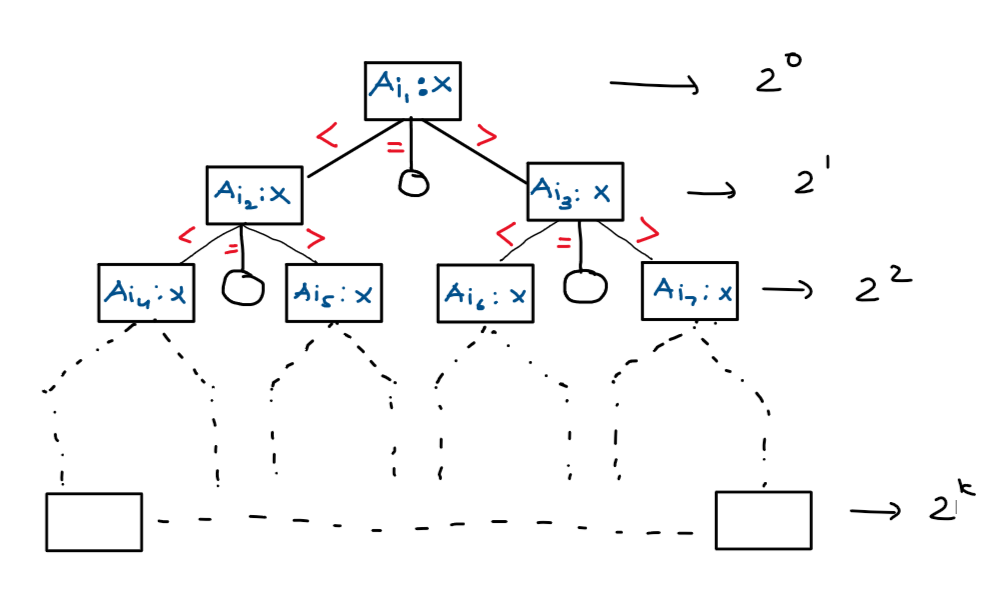
\includegraphics[scale=0.7]{tree.png}
			\linebreak
			As shown in the above tree, at each node of the tree we are making comparison of $A_{i_k}$th element of the array with $x$. Based on the three possible results of each combination we are going down the tree. There has to be at least $n$ nodes to make these comparisons. (Since there are $n$ elements in the array, if we are comparing less than $n$ times, there is a possiblity that the element of the array with which we did not compare $x$ with turns out to be equal to $x$), hence there has to be at least $n$ leaves in total in the tree. This is a complete binary tree, hence at level $k$, the number of nodes are equal to $2^{k-1}$, if we consider root to be at level 1.\\ 
			$$\therefore \sum_{i=1}^{k}2^{i-1} \geq n$$
			$$\therefore 2^{k}-1 \geq n$$
			$$\implies k \geq \log{n}$$
			To search for any $x$ in any sorted array we will have to go through a path with $k$ nodes hence at least $\log{n}$ nodes. One node is one comparison hence we will have to make at least $\log{n}$ comparisons. Since the worst case time complexity of binary search is also $\mathcal{O}(\log n)$ we can say that binary search is optimal.\\
			\linebreak
			Since, we have already found the worst case time complexity for searching algorithm we will find the average case time complexity. To do this we will try to find the expected value of number of comparisons required. In a way, if $X$ is a random variable that describes number of comparisons required to find $x$. At level $l$ probability of finding $x$ would be $\frac{2^{l-1}}{2^k - 1}$, where $k$ is the total number of levels. In a way $X =$ level at which $x$ was found. So, the expected value of number of steps required can be calculated as:
			\begin{align*} 
				\mathbb{E}[X] &\geq \sum_{l=1}^{k}l.\mathbb{P}(X=l) &\\
				&\geq \sum_{l=1}^{k}l.\frac{2^{l-1}}{2^k - 1} &\\
				&\geq \frac{1}{2^k - 1}\sum_{l=1}^{k}l.2^{l-1} &\\
			\end{align*}
			To solve, the summation, let 
			\begin{equation}\label{eq-1}
				S = 1.2^{0} + 2.2^{1} + 3.2^{2} \dots + k.2^{k-1}\\
			\end{equation}
			\begin{equation}\label{eq-2}
				2S = 1.2^{1} + 2.2^{2} \dots + (k-1).2^{k-1} + k.2^{k}\\
			\end{equation}
			Substracting \ref{eq-2} from \ref{eq-1} we get, 
			\begin{flalign*}
				-S = 1.2^0 + 2^1 + 2^2 + \dots + 2^{k-1} - k2^k\\
				-S = 2^k - 1 - k2^k\\
				S = k2^k - (2^k - 1)\\
				\implies S \geq n\log{n} - n
			\end{flalign*} 
			Hence, by the equations above we have,
			\begin{align*}
				\mathbb{E}[X] &\geq \frac{1}{n}(n\log{n} - n) &\\
				&\geq \log{n} - 1 &\\
				&\geq \log{n} &\\
			\end{align*}
		Hence, the average time complexity of the any search algorithm is $\mathcal{O}(\log{n})$.
		\newpage
		
	\section*{\underline{Q-3}}
		Given below is the implementation of heap-sort algorithm in C++:
		\begin{lstlisting}[language=C++]
			void max_heapify(vector<int> &A, int i, int n){
				int left = 2*i;
				int right = 2*i + 1;
				int largest = i;
				if(left < n && A[left] > A[i]){
					largest = left;
				}
				if(right < n && A[right] > A[largest]){
					largest = right;
				}
				if(largest != i){
					swap(A[i], A[largest]);
					max_heapify(A, largest, n);
				}
			}
			
			void build_max_heap(vector<int> &A){
				int n = A.size();
				for(int i=n/2; i>=0; i--){
					max_heapify(A, i, n);
				}
			}
			
			void heapsort(vector<int> A){
				build_max_heap(A);
				int k = A.size();
				int n = k;
				for(int i=0; i<A.size()-1; i++){
					
					// Swap the root with the last element
					// Basically are putting the maximum element to its correct place
					swap(A[0], A[n-i-1]);
					
					// We make a max-heap of the remaining elements and repeat the process
					max_heapify(A, 0, --k);
				}
			}
		\end{lstlisting}
		
		To give the proof of correctness of heapsort, in this particular question, I will be skipping proof of correctness for max-heapify and build-max-heap functions and only focus on heapsort. We will assume max-heapify and build-max-heap to be black boxes for this problem.\\
		For proof of correctness we will take the following loop invariant : "Before the $j$th iteration of the algorithm , the elements of array $A[1 \dots n-j+1]$ will be a max-heap and the array $A[n-j+2\dots n]$ will contain the largest elements and they will be sorted".\\
		\linebreak
		\textbf{\underline{Proof}}\\
		\linebreak
		\textbf{Initialization : }Before the first iteration $j = 1$, hence the array $A[1\dots n-j+1]$ should be a max-heap. As it can be seen from the code, in our function heapsort, we are building a max-heap with the original unsorted array $A$. Hence, initialization holds true.\\
		\textbf{Maintenence : }Let us assume that our property holds before the $j$th iteration, we now need to prove that the property holds true for the $j+1$th iteration as well. Since property was true before the $j$th iteration it means that the array $A[1\dots n-j+1]$ is a max-heap and the array $A[n-j+2/dots n]$ contains the largest elements of the array which are sorted. Now in the $j$th loop we are first of all swapping the last element of the max-heap $A[1\dots n-j+1]$ with first element. Since the first element of a max-heap is the maximum of that array, $A[i] > A[t], \forall t \leq n-j+1, t \neq 1$. Now, we build a heap for the elements from $A[1\dots n-j]$. This means that we have extracted the highest element from the array $A[1\dots n-j+1]$. \\
		Hence, in the next iteration, we can observe that the array $A[1\dots n-j]$ is a max-heap and the array $A[n-j+1\dots n]$ is sorted.\\
		\linebreak
		\textbf{Termination : }Termination step states that our array $A[1\dots 1]$ (because $j=1$) is a max-heap having the smallest elements and the array $A[2\dots n]$ contains the largest elements of the array in sorted fashion. This itself implies that our array $A$ is sorted.  
		
	\section*{\underline{Q-5}}
		This question can be easily solved by using recursion and traversing through subtress. This is a simple problem where we will use divide and conquer to compare $x$ with $k$ elements and terminate when more than $k$ elements have already been compared. Why do we do this? We do it because we have to check whether $k$th smallest element is bigger than $x$. If it is, then it implies that there are at most $k-1$ elements smaller than $x$. If there are more than $k-1$ elements smaller than $x$ in the min-heap then we know that $x$ would be greater than equal to the $k$th smallest element. The C++ code for the problem is as follows:
		\begin{lstlisting}[language=C++]
			vector<int> heap;
			int x, k, values_smaller;
			
			// Recursively check for each subtree
			void check(int i){
				if(heap[i] < x){
					values_smaller++;
					
					// If already k values smaller than x are discovered then we stop 
					// If we reach the leaf nodes, we stop
					if(values_smaller < k && (2*i + 1) < heap.size()){
						// Check for left subtree
						check(2*i);
						
						// Check for right subtree
						check(2*i + 1);
					}
					else{
						return;
					}
				}
			}
			
			// Runner function
			bool runner(){
				values_smaller = 0;
				check(0);
				if(values_smaller >= k){
					return false;
				}
				return true;
			}
		\end{lstlisting}
		\textbf{Proof of Correctness : }Since we are given a min-heap, for any tree, the depth first traversal will yield larger values after each step, (the children values will be greater than the parent values). This means that our algorithm stops once it discovers $heap[i] \geq x$. Thus the recursion happens at most $2*k$ times in the worst case (It happens when we $k$th element of a subtree turns out to be smaller than k). This means our worst time complexity is $\mathcal{O}(k)$.\\
		If the $k$th smallest element is really greater than $x$, then total traversals on the left subtree from the root and right subtree from the root should sum to $k-1$ or smaller. This check is made at the if condition in the code. If it does not happen then we know for sure that the $k$th smallest element is not bigger than $x$ and there are more than $k-1$ values in the min-heap smaller than $x$ (The check for this is given in the if condition of runner function).
		
	
\end{document}